\chapter{Ricerca degli zeri di una funzione}

\section{Introduzione}

La determinazione degli zeri di una funzione, ovvero la risoluzione dell'equazione $f(x) = 0$, costituisce uno dei problemi fondamentali dell'analisi numerica. Nonostante la formulazione apparentemente semplice, si tratta in generale di un problema non banale quando non si ha una soluzione analitica.

L'idea di base è la seguente: si cerca inizialmente di individuare in maniera approssimata una regione dello spazio in cui è presente uno zero della funzione; successivamente si utilizza un algoritmo numerico per raffinare progressivamente la stima.


\paragraph{Esempio introduttivo:}

\begin{multicols}{2}
Consideriamo la funzione

\[
f(x) = x + \frac{x^2}{10},
\]

e supponiamo di studiarla nell'intervallo

\[
[-15,\,10].
\]

Un primo approccio consiste nel valutare la funzione in un numero finito di punti (ad esempio 30 punti equispaziati) e osservare il comportamento del grafico. 

\begin{figure}[H]
	\centering
	\label{es1}
	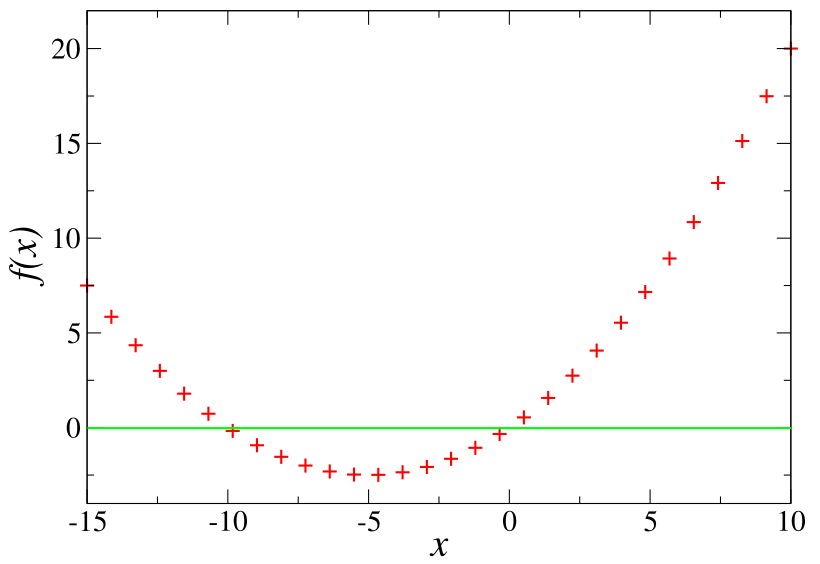
\includegraphics[width=7.2cm]{img/roots1.png}
	\caption{esempio di funzione $f(x)$ plottata con soli 30 punti per stimare i segmenti in cui cercare lo zero.}
\end{figure}

\end{multicols}

Questo permette di individuare visivamente la regione in cui la funzione cambia segno, e quindi dove è presente uno zero.

Questa fase preliminare è essenziale: senza una buona stima iniziale della posizione dello zero, molti metodi numerici risultano inefficaci o addirittura divergenti.

\paragraph{Casi difficili e comportamenti patologici:}

Esistono tuttavia funzioni per le quali la localizzazione dello zero può risultare estremamente complicata dal punto di vista numerico.

\begin{multicols}{2}
Un esempio significativo è dato dalla funzione

\[
f(x)\ =\ 3x^2\, +\, 1\, +\, \frac{\ln\left[(\pi - x)^2\right]}{\pi^4}.
\]

In questo caso esistono due zeri situati approssimativamente in

\[
x\ \approx\ \pi\, \pm\, 10^{-667}.
\]

\begin{figure}[H]
	\centering
	\label{es2}
	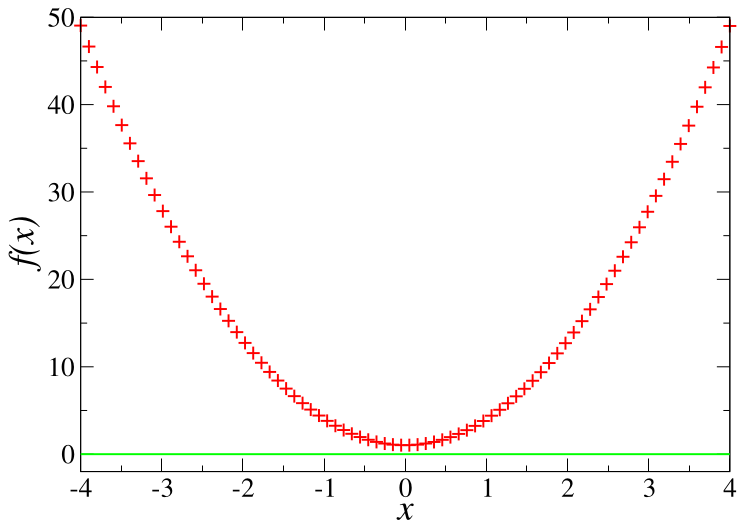
\includegraphics[width=7cm]{img/roots2.png}
	\caption{Funzione $f(x)$ plottata con 80 punti nel range [-4; 4]}
\end{figure}

\end{multicols}

Si tratta di zeri estremamente vicini al valore \( \pi \), tanto che una loro individuazione diretta tramite semplice campionamento risulta praticamente impossibile.

Tuttavia, osservando la struttura della funzione, si nota che il termine logaritmico diventa molto grande e negativo quando \( x \) si avvicina a \( \pi \). Questo suggerisce che lo zero si trovi nelle vicinanze di tale punto.

Questo esempio mostra chiaramente come, in molti casi, sia necessario combinare osservazioni qualitative sulla funzione con tecniche numeriche.

Nel seguito assumeremo di essere riusciti a individuare un intervallo che contiene uno zero della funzione e ci concentreremo su come raffinarne la posizione.

\section{Metodo di bisezione}

Una volta individuato un intervallo in cui è presente uno zero, il metodo più semplice per determinarlo con precisione è il \textbf{metodo di bisezione}.

Questo metodo si basa su una proprietà fondamentale delle funzioni continue: se una funzione cambia segno in un intervallo, allora deve necessariamente annullarsi in almeno un punto interno.

\paragraph{Idea del metodo}

Supponiamo di conoscere due punti \( x_1 \) e \( x_2 \) tali che la funzione cambia segno nell'intervallo \([x_1, x_2]\), ovvero:

\[
f(x_1) > 0, \qquad f(x_2) < 0,
\]

Si definisce quindi il punto medio $x_m = \frac{x_1 + x_2}{2}$ e si valuta il segno della funzione nello stesso:

\begin{itemize}
	\item se \( f(x_m) > 0 \), lo zero si trova nell'intervallo \([x_m, x_2]\), quindi si pone \( x_1 = x_m \);
	\item se \( f(x_m) < 0 \), lo zero si trova nell'intervallo \([x_1, x_m]\), quindi si pone \( x_2 = x_m \).
\end{itemize}

Il procedimento viene quindi iterato, restringendo progressivamente l'intervallo che contiene lo zero.

\paragraph{Stima dell'errore: }

Se inizialmente la lunghezza dell'intervallo è $\epsilon = |x_1 - x_2|$, dopo $n$ iterazioni la lunghezza dell'intervallo si riduce a $\delta \,\approx\,\epsilon\,/\,2^n$.

Questo fornisce una stima diretta dell'errore sulla posizione dello zero.

\paragraph{Esempio numerico del metodo di bisezione: }

Consideriamo la funzione

\[
f(x) = \frac{x^3}{5} + \frac{x}{5} + 0.1.
\]

Applicando il metodo di bisezione si ottiene la seguente sequenza di approssimazioni:

\begin{center}
	\begin{tabular}{c c c}
		\hline
		$i$ & $x_r$ & $\delta$ \\
		\hline
		1 & -0.9   & 0.9  \\
		2 & -0.45  & 0.45 \\
		3 & -0.23  & 0.23 \\
		4 & -0.338 & 0.11 \\
		5 & -0.394 & 0.06 \\
		6 & -0.422 & 0.03 \\
		\hline
	\end{tabular}
\end{center}

Si osserva come l'intervallo contenente lo zero si restringa progressivamente e la stima della radice converga.

\bigskip

Questo esempio illustra chiaramente il comportamento del metodo: la convergenza è garantita, ma relativamente lenta, poiché l'errore si riduce esponenzialmente con fattore \(1/2\) ad ogni iterazione.

\subsection{Osservazioni sul metodo di bisezione}

Il metodo di bisezione è estremamente robusto e presenta alcune caratteristiche fondamentali, esso converge purché la funzione sia continua e si riesca a individuare un intervallo in cui essa cambia segno. Tuttavia, la convergenza è relativamente lenta, in quanto l'errore si riduce secondo la legge $ \delta\, =\, \epsilon/2^n$. 

\begin{multicols}{2}
	
	\begin{figure}[H]
		\centering
		\label{zeri}
		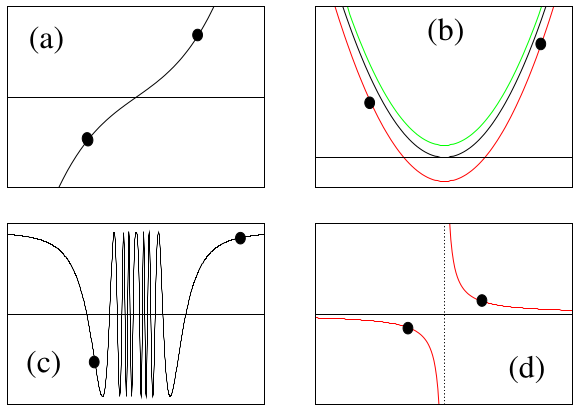
\includegraphics[width=7cm]{img/roots14.png}
		\caption{Casi particolari che si possono verificare.}
	\end{figure}
	
	Esistono diversi casi particolari che è opportuno considerare:
	
	\begin{itemize}
		\item \textbf{Caso normale}: la funzione cambia segno una sola volta nell'intervallo e il metodo converge allo zero corretto.
		\item \textbf{Radici multiple}: la funzione può toccare l'asse senza cambiare segno; in questo caso il metodo può non individuare correttamente lo zero.
		\item \textbf{Radici molto vicine}: possono esistere più zeri estremamente vicini tra loro, rendendo difficile l'identificazione numerica.
		\item \textbf{Discontinuità}: se la funzione presenta una discontinuità, il metodo converge comunque, ma al punto di discontinuità anziché a uno zero reale.
	\end{itemize}
	
	
\end{multicols}


%
%
%
\section{Metodo di Newton-Raphson}

Un approccio più sofisticato per il raffinamento della radice è il metodo di \textbf{Newton-Raphson}: supponiamo di avere una stima iniziale \( x \) della radice e di voler trovare una stima migliorata \( x_r \). Si approssima la funzione tramite lo sviluppo di Taylor al primo ordine:

\[
f(x_r)\ \approx\ f(x)\, +\, (x_r - x)\, \frac{df(x)}{dx} \ \overset{!}{=}\ 0\ \ .
\]

Imponendo la condizione \( f(x_r) \overset{!}{=} 0 \), da cui segue immediatamente

\begin{equation}
	\label{Newton-Raphson}
	x_r\ =\ x\, -\, \frac{f(x)}{f'(x)}.
	\quad \Rightarrow \quad 
	x_{i+1}\ =\ x_i\, -\, \frac{f(x_i)}{f'(x_i)}\ \ .
\end{equation}

Questa relazione definisce una procedura iterativa.

\paragraph{Esempio numerico: }

Consideriamo nuovamente la funzione $f(x) = \frac{x^3}{5} + \frac{x}{5} + 0.1\  .$

\begin{multicols}{2}
	
	\begin{figure}[H]
		\centering
		\label{NewtonCotes}
		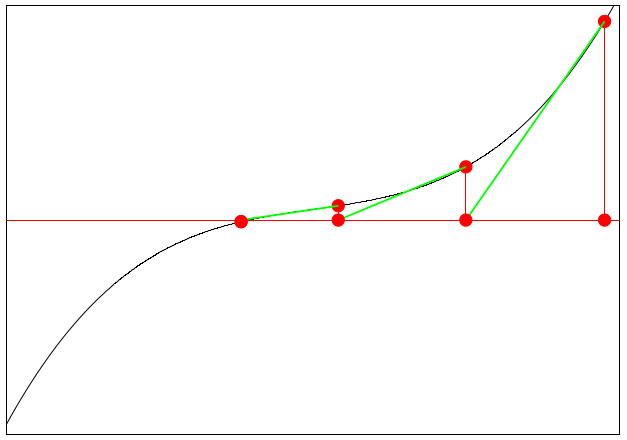
\includegraphics[width=7cm]{img/roots15.png}
	\end{figure}
	
	Applicando il metodo di Newton-Raphson si ottiene la seguente sequenza:
	
	\begin{center}
		\begin{tabular}{c c c}
			\hline
			$i$ & $x_r$ & $f(x_r)$ \\
			\hline
			0 & 1.9    &  \\
			1 & 1.1173 & 0.60 \\
			2 & 0.4825 & 0.22 \\
			4 & -0.4714 & 0.02 \\
			5 & -0.4257 & 0.0006 \\
			7 & -0.4239 & < $10^{-8}$ \\
			\hline
		\end{tabular}
	\end{center}

\end{multicols}

Si osserva una convergenza molto più rapida rispetto al metodo di bisezione.

\subsection{Analisi dell'errore}

Per comprendere meglio la velocità di convergenza, consideriamo una radice \( x_r \) e poniamo $x = x_r + \epsilon$ , così che sviluppando la funzione:

\[
f(x + \epsilon)\ =\ f(x)\, +\, \epsilon\, f'(x)\, +\, \frac{\epsilon^2}{2}\, f''(x)\ \ .
\]

Stavolta non buttiamo via il termine del secondo ordine così applicando l'iterazione di Newton-Raphson di eq.(\ref{Newton-Raphson}) si ottiene una stima per l'errore:

\[
\epsilon_{i+1} = - \frac{\epsilon_i^2 f''(x_i)}{2 f'(x_i)}.
\]

Questo mostra che l'errore si riduce \textbf{quadraticamente}, ovvero

\[
\epsilon_{i+1} \sim \epsilon_i^2,
\]

il che spiega la rapidissima convergenza del metodo.

\subsection{Osservazioni sul metodo di Newton-Raphson}

Il metodo di Newton-Raphson presenta numerosi vantaggi:

\begin{multicols}{2}
\begin{itemize}
	\item convergenza molto rapida;
	\item esatto per funzioni lineari;
	\item estendibile a più dimensioni;
	\item non richiede il bracketing della radice.
\end{itemize}
\end{multicols}

Tuttavia presenta anche alcune criticità:

\begin{multicols}{2}
\begin{itemize}
	\item richiede una buona stima iniziale, altrimenti...
	\item ... può divergere o oscillare;
	\item può bloccarsi in punti stazionari;
	\item fallisce in presenza di discontinuità;
	\item richiede che \( f'(x) \neq 0 \).
\end{itemize}
\end{multicols}
	
	
\begin{figure}[H]
		\centering
		\label{newton cotes comments}
		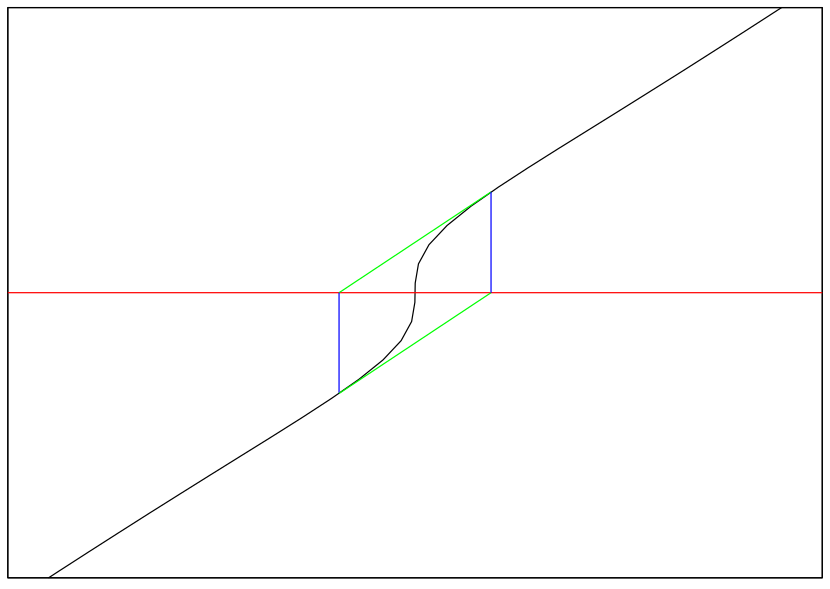
\includegraphics[width=6cm]{img/roots16.png}
		\caption{esempio visivo di radice che fa andare in palla il metodo di Newton-Raphson.}
\end{figure}



%
%
%
\section{Caso dei polinomi, metodo di Laguerre}

Nel caso particolare dei polinomi esistono metodi specifici molto efficienti.

Consideriamo un polinomio scritto nella sua forma fattorizzata:

\[
P_n(x)\ =\ (x - x_1)\, (x - x_2)\, \cdots\, ( x - x_n).
\]

Si può portare il prodotto ad essere una sommatoria usando il logaritmo:

\[
\ln |P_n(x)|\ =\ \sum_i\, \ln |x - x_i|.
\]

Derivando:

\[
\frac{d}{dx} \ln |P_n(x)|\ =\ \sum_i\, \frac{1}{x - x_i}\
=\ \frac{P'_n(x)}{P_n(x)}\ \equiv\ G,
\]

Questa nuova quantità $G$ possiamo trattarla come una grandezza che ci dice in base al punto $x$ in cui siamo quanto siamo vicini a ciascuna radice (vedi l'inverso, se siamo molto vicini, $G$ diventa molto grande). In particolare la radice più vicina $x_k$ contribuirà molto di più nella sommatoria, quindi $x_k\approx x - \frac{1}{G}$ in prima approssimazione.

\[
\frac{d^2}{dx^2} \ln |P_n(x)|\ =\
\sum_i\, \frac{1}{(x - x_i)^2}
\ =\ \left[\frac{P'_n}{P_n}\right]^2\, -\, \frac{P''_n}{P_n}\ =\ H.
\]

Possiamo esprimere H in funzione del polinomio e di G, che porta informazioni sulla distanza delle radici: $H=G^2 - P_n ''/P_n$  .

Si ottiene quindi $G\,=\, \frac{1}{a} + \frac{n-1}{b}$ e $H\,=\, \frac{1}{a^2} + \frac{n-1}{b^2}$, dove in particolare $a$ è la distanza della radice più vicina ($a=x-x_k$) e $b$ è la distanza di 'tutte' le altre radici (facendo finta siano tutte ugualmente distanti, $\sum_{i\neq k} (x - x_i)^{-2}\approx\frac{n-1}{b}$), così abbiamo una prima stima infine della distanza della radice:

\[
a = \frac{n}{G \pm \sqrt{(n-1)(nH - G^2)}}.
\]

Il metodo consiste nell'iterare $x \rightarrow x - a$ , scegliendo il segno che massimizza il denominatore.

%
%
%
\vspace{0.5cm}
\section{Generalizzazione a più dimensioni di Newton-Raphson}

Il problema della ricerca degli zeri si estende naturalmente a più dimensioni.

Si considerano sistemi del tipo $f_i(\mathbf{X}) = 0$, con $i=1,\dots , n$, dove \( \mathbf{X}=(x_1,\, \dots ,\, x_n) \) è un vettore in \( \mathbb{R}^n \).

Si generalizza il metodo di Newton-Raphson scrivendo

\[
f_i(\mathbf{X} + \delta)\ \approx\ f_i(\mathbf{X})\, +\, \sum_j\, \frac{\partial f_i}{\partial x_j}\, \delta_j.
\]

Definendo $a_{ij} = \frac{\partial f_i}{\partial x_j}$, coefficienti dello jacobiano, si ottiene il sistema lineare:

\[
\sum_j\, a_{ij}\, \delta_j\ =\ -f_i(\mathbf{X}).
\]

Risolvendo per \( \delta \) si ottiene  $\delta_j = - \sum_i (a_{ij})^{-1} f_i(\mathbf{X})$  e si itera seguendo  $X_i^{(\text{new})} = X_i^{(\text{old})} + \delta_i$  .

\begin{multicols}{2}
\paragraph{Esempio bidimensionale: }

Un esempio di sistema non lineare è

\[
f_1(x,y) = x^2 + y^2 - 1,
\]

\[
f_2(x,y) = y - x^2 + \frac{x}{2}.
\]

La soluzione corrisponde all'intersezione delle due curve.

\begin{figure}[H]
	\centering
	\label{esempio bidi}
	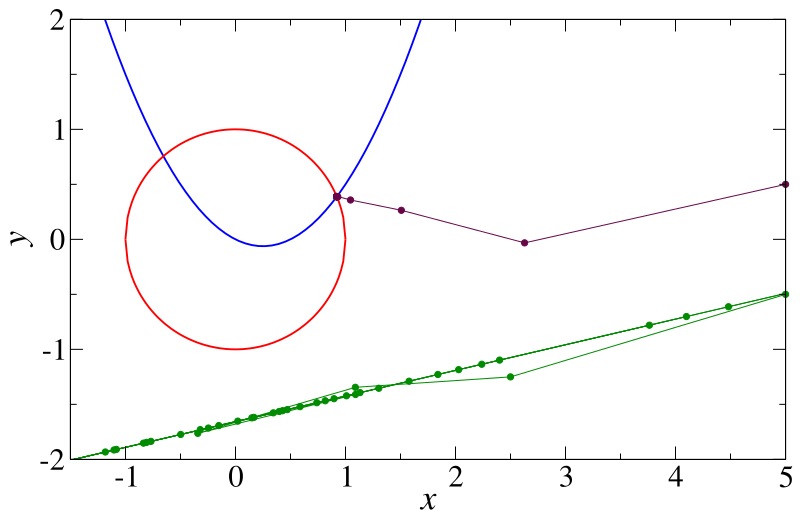
\includegraphics[width=6cm]{img/roots18.png}
	\caption{esempio bidimensionale}
\end{figure}

\end{multicols}

\section{Conclusioni}

Riassumendo:

\begin{itemize}
	\item è sempre necessario avere un'idea preliminare della posizione della radice;
	\item il metodo di bisezione è robusto ma lento;
	\item il metodo di Newton è rapido ma delicato;
	\item per i polinomi esistono metodi dedicati;
	\item in più dimensioni il metodo di Newton è lo strumento principale, ma è sensibile alle condizioni iniziali.
\end{itemize}

\bigskip

La scelta del metodo più adatto dipende quindi dal problema specifico, dal grado di informazione disponibile sulla funzione e dal compromesso desiderato tra stabilità e velocità di convergenza.